\chapter{Erweiterte Funktionen}
\section{Das \tag-Konzept von PUMA}

\subsection{\tags}
\label{subsec:tags}
\tags\index{Tags} (dt. Schlagwörter) ermöglichen ein übersichtliches Organisieren und Strukturieren der Lesezeichen. Einem Literatureintrag können beliebig viele \tags zugeordnet werden. Durch den Gebrauch von \tags wird die Suche zu einem bestimmten Thema erleichtert, da nach den \tags gezielt gesucht werden kann (\autoref{Suche}). \\
\begin{figure}[h!]
 \centering
 \fbox{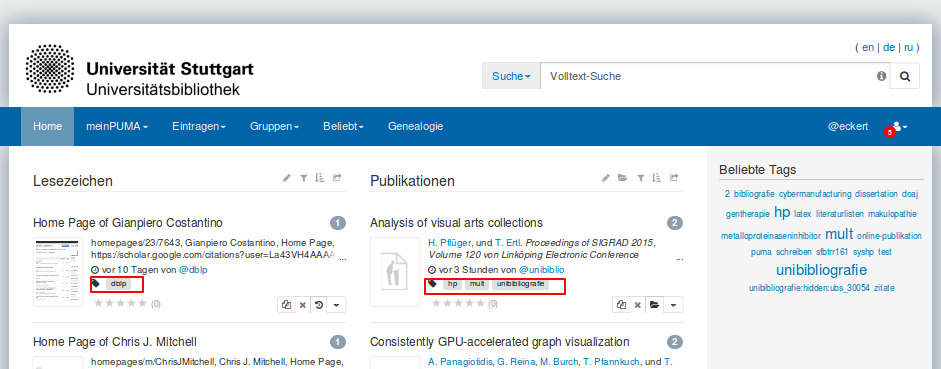
\includegraphics[width=10cm]{Bilder/Kapitel6/Tags}}
 \caption{Tags}
 \label{figure025}
\end{figure}
\textbf{\tags zu Lesezeichen/~Publikationen hinzufügen}\newline
Jeder neue Eintrag braucht mindestens ein \tag. Es können beliebig viele \tags, durch Leerzeichen getrennt, hinzugefügt werden. Beim BiBTeX-Export werden nur bei den eigenen Einträgen die \tags im Feld keywords exportiert.\\
\begin{figure}[h!]
 \centering
 \fbox{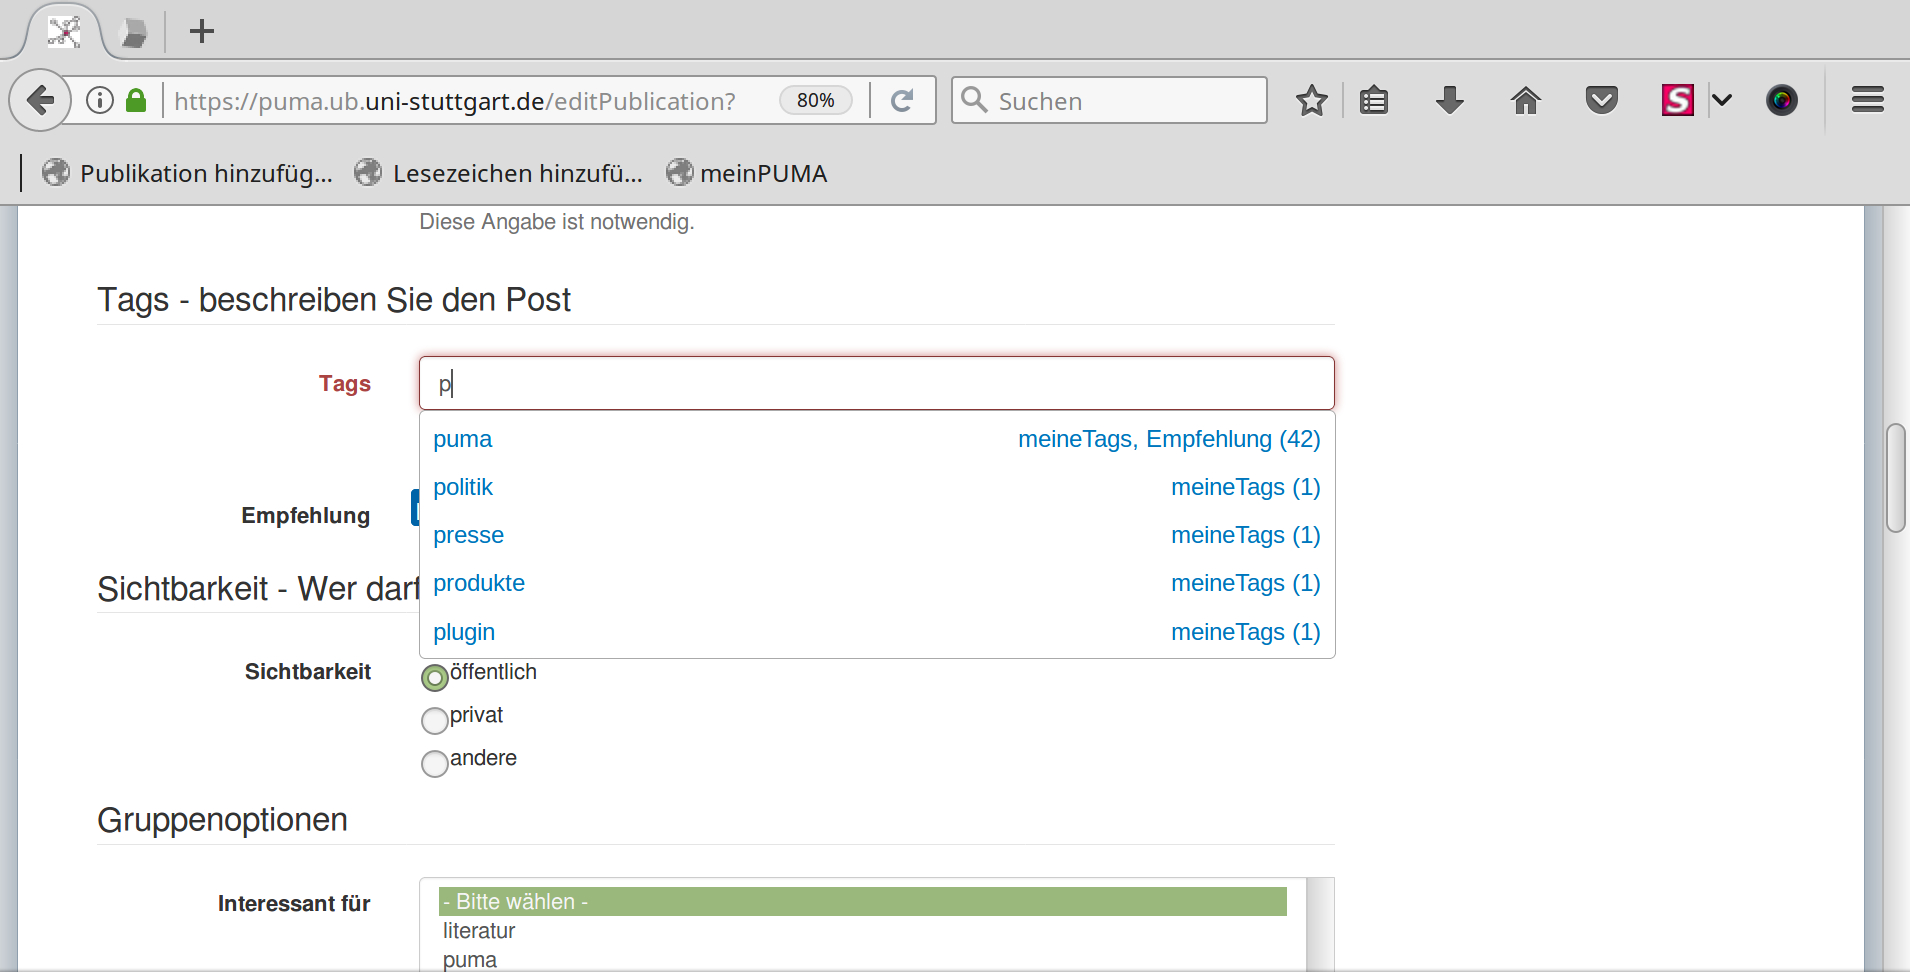
\includegraphics[width=10cm]{Bilder/Kapitel6/Tags_hinzufuegen}}
 \caption{Tags hinzufügen}
 \label{figure026}
\end{figure} 
%\begin{wrapfigure}{l}{7cm}
%\end{wrapfigure}
\textbf{\tags von Lesezeichen/~Publikationen bearbeiten} \newline
PUMA bietet drei Möglichkeit bei Publikationen/~Lesezeichen, die schon Teil einer Sammlung sind, die \tags zu bearbeiten: \index{Tags!bearbeiten}
\begin{itemize}
    \item \underline{\enquote{Schnellbearbeitung}}\newline
   Über das blaue Stiftsymbol (\enquote{\tags bearbeiten}) vor den vorhandenen \tags können diese gelöscht (\enquote{X-Symbol} im blau hinterlegten\tag oder neue hinzuzufügt werden. Dazu im Textfeld die \tags durch Leerzeichen getrennt eingeben.
    \item \underline{über \enquote{Eintrag bearbeiten}}\newline
    Über die Bearbeitungsfunktion der gesamten Publikation, können auch die \tags angepasst werden. \todo[inline]{Querverweis}
    \item \underline{mehrere \tags bearbeiten}\newline
    PUMA bietet die Möglichkeit alle verwendeten \tags zu bearbeiten. Dazu über das Personensymbol\enquote{Tags bearbeiten} auswählen und eine der folgenden Aktion durchführen:
    \begin{enumerate}
        \item Umbenennen/~Ersetzten von Tags: \newline Hier können \tags ersetzt werden. So z.B. ähnliche \tags zu einem \tag zusammengefügt werden.
        \item Subtags zu Konzepten hinzufügen: \newline
        Um ein Subtag zu einem Konzept hinzuzufügen, den Namen des Konzepts in das Feld \enquote{Supertag} eingeben und das \tag, das hinzufügt werden soll in das Feld \enquote{Subtag}. Anschließend auf \enquote{Einfügen} klicken (\autoref{subsec:Konzepte}).
        \item Subtags von Konzepten löschen:\newline Um ein Subtag von einem Konzept zu löschen, den Namen des Konzepts in das Feld \enquote{Supertag} und das zu löschende \tag, in das Feld \enquote{Subtag} eingeben. Anschließend auf \enquote{Löschen} klicken.
    \end{enumerate}
\end{itemize}
\textbf{Suchen\index{Suche} via Tags}\newline
PUMA ermöglicht, dass Sie mit Hilfe der Tags Lesezeichen und Publikationen finden können. \newline\newline
\underline{Möglichkeit 1:} Um einen Eintrag mit einem bestimmten Tag zu finden klicken Sie in der Suchleiste neben \enquote{Suche} auf den blauen Pfeil und wählen im Dropdown-Menü \enquote{Tags} aus. Geben Sie den Tag in das Suchfeld ein und drücken auf das Lupensymbol oder die Enter-Taste.\newline \newline
\underline{Möglichkeit 2:} Wenn Sie bei einem Eintrag auf einen Tag klicken, öffnet sich eine Seite mit allen Einträgen des Nutzer mit diesem bestimmten Tag. Auf der rechten Seite sehen Sie Informationen zu diesen Tag: Der Tag als Tag von allen Nutzern, verwandte Tags, die Konzepte des Nutzers und die verwendeten Tags des Nutzers. 
\newline
\newline
\subsubsection*{Systemtags\index{Systemtags}}
Systemtags\index{Tags!Systemtags} \label{systemtag} sind spezielle Tags, die eine feste Bedeutung haben. Derzeit bietet PUMA drei Typen von Systemtags an:
\begin{description}
\item[Ausführbare Systemtags:]
Ausführbare Systemtags werden zu einem Eintrag hinzugefügt, um eine spezielle Aktion mit diesem Eintrag auszuführen. Sie tragen ausführende Systemtags, wie die anderen Tags, in das Feld \enquote{Tags} ein. 
\begin{enumerate}
    \item \textit{for:<Gruppenname>} : Mit diesem Systemtag kopieren Sie den Eintrag in die Sammlung der Gruppe. In der Gruppe wird der Tag durch \textit{from:<IhrBenutzername>} ersetzt. Wenn Sie ihren Eintrag löschen oder bearbeiten, so bleibt der in die Gruppe kopierte Eintrag unverändert. Nur Mitglieder der Gruppe können Einträge für die Gruppe kopieren.
    \item \textit{send:<Benutzername>} : Damit senden Sie den Eintrag in den Eingang eines anderen Benutzers. Damit dies funktioniert, muss der Empfänger Sie als Freund eingetragen haben oder Sie müssen Mitglied in der gleichen Gruppe sein. Sobald der Eintrag bei dem Nutzer angekommen ist wird der Tag durch \textit{sent:<Benutzername>} ersetzt.
\end{enumerate}
\item[Meta-Systemtags:]  
Mit Meta-Systemtags markieren Sie Einträge. Derzeit werden folgende Meta-Systemtags unterstützt:
\begin{enumerate}
    \item \textit{myown:} Ein Eintrag, der mit dem Tag myown\index{myown} versehen wurde, erscheint auf Ihrer CV-Seite. Durch den Tag geben Sie an, dass Sie der Verfasser des Lesezeichen/der Publikation sind.
    \item \textit{sys:relevantFor:<Gruppenname>} : Einträge mit dem Tag sys:relevantFor:xy werden auf der \enquote{Interessant für\index{Interessant für}}-Seite der Gruppe xy angezeigt. Damit hat dieser Tag den gleichen Effekt, wie das  Auswählen der Gruppe xy in der \enquote{Interessant für}-Box beim Bearbeiten eines Eintrages. Der Tag wird durch eine blaue Blume am Anfang der Tag-Reihe dargestellt. 
    \item \textit{sys:hidden:<tag>} : Der Tag ist nur für Sie selbst sichtbar. Man findet diesen Tag bei einer Publikation, die im Inhaltsbereich abgebildet wird, nicht sichtbar in der Reihe der anderen Tags. Der Tag wird durch eine blaue Blume am Anfang der Tag-Reihe dargestellt. Wenn Sie auf die Detailansicht der Publikation klicken, taucht er sichtbar in der Tag-Reihe auf.
\end{enumerate}
\item[Such-Systemtags:] 
\label{itm:suchSystemtag}
Such-Systemtags sind nicht dazu da, um in einen Eintrag geschrieben zu werden, sondern um Einträge nach Suchanfragen zu filtern. Alle Such-Systemtags haben die gleiche Syntax: \textit{sys:<Feldname>:<Feldwert>}. Beispielsweise werden  bei der Suchanfrage \textit{sys:author:xyz} nur die Einträge angezeigt, welche von dem Autor \textit{xyz} stammen.\newline
Die Syntax kann entweder in die Suchleiste oder mit der URL eingeben werden. Folgende Filter unterstützt PUMA (Suche beschränkt sich auf die Publikationseinträge):\newline
\newline
Für die Suche nach einem bestimmten Autor oder Erscheinungsjahr müssen Sie vorher festlegen, in welchen Einträgen eines Nutzers Sie nach dem Autor oder dem Erscheinungsjahr suchen möchten. Zum Beispiel suchen Sie, wenn Sie diese Daten eingeben: \newline https://puma.ub.uni-stuttgart.de/user/\newline droessler/sys:year:2013 \newline Publikationen aus dem Jahr 2013 in den Einträgen des Nutzers Droessler. 
\begin{enumerate}
    \item \textit{sys:author:<Autorenname>} filtert die Suche nach dem Autor.
    \item \textit{sys:year:<Jahr>} filtert die Suche nach dem Erscheinungsjahr. Dabei sind mehrere Schreibweisen für das Jahr möglich:
    \begin{enumerate}
        \item 2000: Alle Einträge aus dem Jahr 2000
        \item 2000-: Alle Einträge aus dem Jahr 2000 oder einem Jahr danach
        \item -2000: Alle Einträge aus dem Jahr 2000 oder einem Jahr davor
        \item 1990-2000: Alle Einträge aus den Jahren 1990 bis 2000
    \end{enumerate}
%muss noch raus rutschen
Bei der Suche nach Titel, Gruppe, Nutzer, usw. spielt der Nutzer, bei dem Sie suchen keine Rolle. Sie müssen dementsprechend nur den Zusatz tag/ vor die Suchsyntax setzten, zum Beispiel  https://puma.ub.uni-stuttgart.de/tag/sys:entrytype:article. Hier finden Sie nun alle Artikel, die auf PUMA eingetragen wurden.
    \item \textit{sys:title:<title>} sucht nach Einträgen mit diesem Titel.
    \item \textit{sys:user:<user>} sucht nach Einträgen eines Nutzers.
    \item \textit{sys:group:<group>} filtert die Suche nach einer bestimmten Gruppe.
    \item \textit{sys:entrytype:<Eintragstyp>} filtert die Suche nach dem Eintragstypen. Eintragstypen\footnote{\url{https://www.ctan.org/pkg/biblatex?lang=de}} werden verwendet, um BibTex-Einträge nach ihren Typen zu klassifizieren. Derzeit unterstützt Puma folgende Eintragstypen\index{Eintragstypen}: 
    \begin{enumerate}
        \item \textbf{article\index{Article}:} Zeitungs- oder Zeitschriftenartikel\newline
        Erforderliche Felder: Autor, Titel, Zeitschriftentitel, Ausgabennummer, Jahr/Datum 
        \item \textbf{book\index{Book}:} Buch, Monografie mit angegebenem Verlag\newline
        Erforderliche Felder: Autor, Titel, Jahr
        \item \textbf{booklet\index{Booklet}:} Gebundenes Druckwerk, aber ohne Verlag oder Sponsororganisation\newline
        Erforderliche Felder: Autor/Lektor, Titel, Jahr/Datum
        \item \textbf{conference\index{Conference}:} Ein Beitrag zu einer Konferenz, der nicht in einem Konferenzband erschienen ist\newline
        Erforderliche Felder: Autor, Titel, Buchtitel, Jahr/Datum
        \item \textbf{electronic\index{Electronic}:} Elektronische Veröffentlichungen, z. B. eBooks oder Blogeinträge\newline 
        Erforderliche Felder: Autor, Buchtitel, Verlag, Adresse, Jahr
        \item \textbf{inbook\index{Inbook}:} Teil eines Buches, z. B. ein Kapitel oder ein Seitenbereich\newline
        Erforderliche Felder: Autor, Titel, Buchtitel, Jahr/Datum 
        \item \textbf{incollection\index{Incollection}:} Teil eines Buches mit einem eigenem Titel, z. B. Beitrag in einem Sammelband\newline
        Erforderliche Felder: Autor, Titel, Buchtitel, Jahr/Datum
        \item \textbf{inproceedings\index{Inproceedings}:} Artikel in einem Tagungsband bzw. Konferenzband\newline
        Erforderliche Felder: Autor, Titel, Buchtitel, Jahr/Datum
        \item \textbf{manual\index{Manual}:} Technische Dokumentation, Handbuch\newline
        Erforderliche Felder: Autor/Lektor, Titel, Jahr/Datum
        \item \textbf{mastersthesis\index{Mastersthesis}:} Master-, Magister- oder Diplomarbeit\newline
        Erforderliche Felder: Autor, Titel, Art der Arbeit, Institut, Jahr/Datum
        \item \textbf{misc\index{Misc}:} Diesen Eintragstyp können Sie wählen, wenn nichts anderes zu passen scheint. \newline
        Erforderliche Felder: Autor/Lektor, Titel, Jahr/Datum
        \item \textbf{patent\index{Patent}:} Patent\newline 
        Erforderliche Felder: Autor, Titel, Nummer, Jahr/Datum
        \item \textbf{periodical\index{Periodical}:} Ein regelmäßig erscheinendes Werk, z.B. Zeitschrift\newline
        Erforderliche Felder: Lektor, Titel, Jahr/Datum
        \item \textbf{phdthesis\index{Phdthesis}:} Doktor- oder andere Promotionsarbeit\newline 
        Erforderliche Felder: Autor, Titel, Hochschule/Universität, Jahr 
        \item \textbf{presentation\index{Presentation}:} Präsentation, Vortrag auf einer Veranstaltung\newline 
        Erforderliche Felder: Verfasser, Titel, Anlass der Präsentation, Jahr
        \item \textbf{proceedings\index{Proceedings}:} Tagungsband einer Konferenz\newline
        Erforderliche Felder: Titel, Jahr/Datum
        \item \textbf{standard\index{Standard}:} Standard\newline 
        Erforderliche Felder: Autor, Buchtitel, Verlag, Adresse, Jahr 
        \item \textbf{techreport\index{Techreport}:} Bericht einer Hochschule oder einer anderen Institution\newline
        Erforderliche Felder: Autor, Titel, Jahr/Datum
        \item \textbf{unpublished\index{Unpublished}:} Nicht formell veröffentlichtes Dokument\newline 
        Erforderliche Felder: Autor, Titel, Jahr/Datum
    \end{enumerate}
    \item \textit{sys:not:<tag>} filtert die Suche, indem alle Ergebnisse ignoriert werden, die diesen Tag enthalten. An dieser Stelle können Sie auch Platzhalter verwenden, z.B. werden bei sys:not:news\_ 
    alle Ergebnisse ignoriert, die Tags enthalten, die mit news\_
    beginnen.
    \item \textit{sys:bibtexkey:<bibtexkey>} filtert die Suche nach einem bestimmten BibTeX-Schlüssel.
\end{enumerate}
\end{description}
\subsection{Konzepte}
\underline{Was sind Konzepte\index{subsec:Konzepte}?}
\newline
Durch Konzepte können Sie Ihre Tags nach Gruppen ordnen und sich so die Suche erleichtern. Sie haben beispielsweise das Konzept mit dem Supertag\index{Supertag} (Namen) Obst, diesem sind die Subtags\index{Subtag} Banane, Apfel und Kiwi zugeordnet. Wenn Sie nun mit dem Konzept Obst suchen, werden Ihnen automatisch alle Publikationen und Lesezeichen angezeigt, die mit mindestens einem der Subtags getagged wurden. Dies erleichtert Ihre Suche, da oft nach Publikationen/Lesezeichen zu einem bestimmten Thema gesucht wird. 
\newline Ihre angelegten Konzepte finden Sie über das Untermenü von \enquote{mein PUMA}. Um zu den beliebten Konzepten von PUMA zu gelangen klicken Sie im Hauptmenü auf \enquote{Beliebte} und anschließend im Untermenü auf \enquote{Konzepte}. 
\newline
\newline
\underline{Konzepte erstellen}
\newline
Um Konzepte zu erstellen oder zu überarbeiten, klicken Sie auf das Personensymbol auf der rechten Seite. Ein Untermenü öffnet sich und Sie klicken auf Tags bearbeiten. 
\begin{figure}[h!]
 \centering
 \fbox{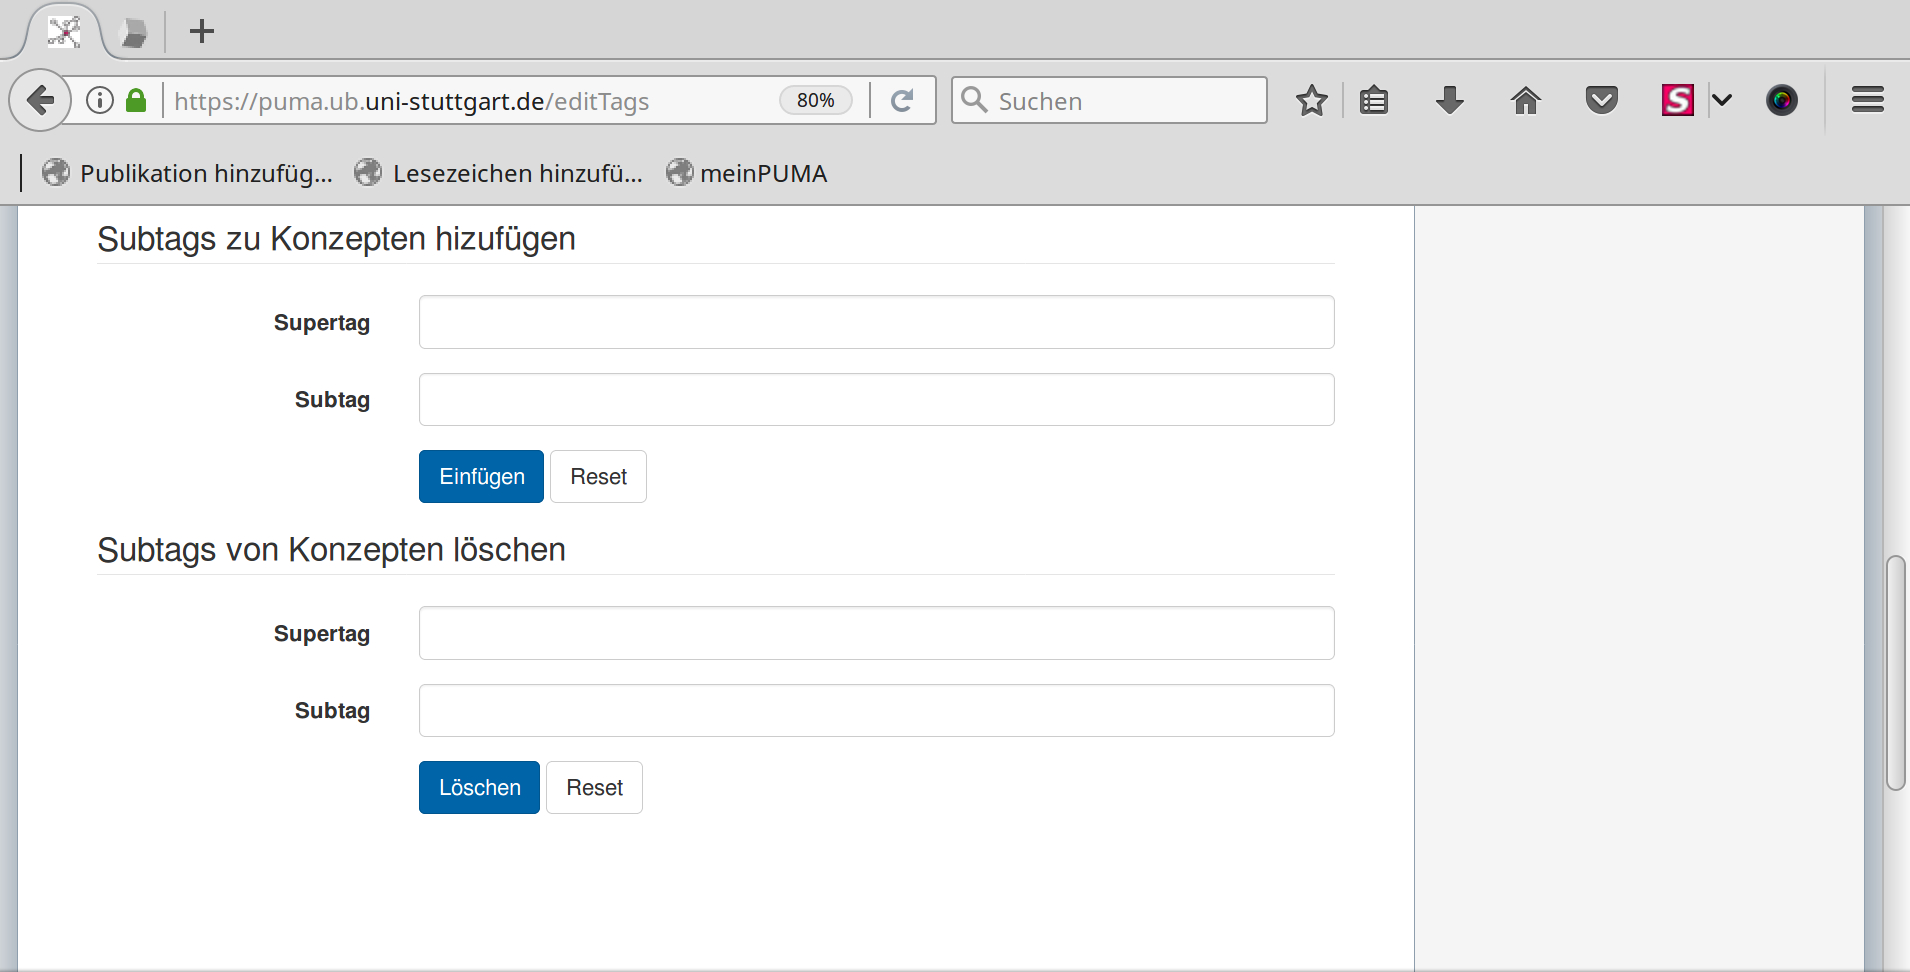
\includegraphics[width=10cm]{Bilder/Kapitel6/Konzepte_erstellen}}
 \caption{Ein Konzept erstellen}
 \label{figure027}
\end{figure}
\textbf{Subtags zu Konzepten hinzufügen:} PUMA ermöglicht Ihnen neue Konzepte zu erstellen oder zu einem bereits existierenden Konzept neue Tags hinzufügen. Um ein neues Konzept hinzuzufügen, wählen Sie einen Tag, der als Name für das Konzept stehen soll, aus. Diesen Tag geben Sie in das Feld \enquote{Supertag} ein. Den Tag, der dem Konzept hinzugefügt werden soll, geben Sie in das Feld \enquote{Subtag} ein.
\begin{mdframed}[style=mdfexample1,frametitle={\texttt{ACHTUNG}},backgroundcolor=gray!40]\texttt{Es kann immer nur ein Subtag eingegeben werden, wenn Sie zwei Subtags gleichzeitig eingeben wird das Konzept nicht erstellt. Um mehrere Subtags in einem Konzept zu vereinen, müssen sie den oben genannten Ablauf zur Erstellung eines Konzeptes mit jedem neuen Subtag wiederholen und dabei das Supertag unverändert lassen.} 
\end{mdframed}
\textbf{Subtags von Konzept löschen:} Sie können auch Tags aus einem Konzept entfernen. Dafür geben Sie in das Feld \enquote{Supertag} den Namen des Konzepts ein und in das Feld \enquote{Subtag} den Tag, der gelöscht werden soll. 
\begin{mdframed}[style=mdfexample1,frametitle={\texttt{ACHTUNG}},backgroundcolor=gray!40]\texttt{Hier kann ebenfalls immer nur ein Tag in das Feld Subtag eingegeben werden, da sonst die Aktion nicht durchgeführt wird.}
\end{mdframed}
\underline{Navigation mit Konzepten}
\newline
Um mit Konzepten zu suchen, benutzen Sie einfach die Suchleiste rechts oben. Klicken Sie auf den blauen Pfeil neben \enquote{Suche} und wählen Sie im Dropdown-Menü Konzepte aus. Geben Sie den Namen des Konzepts, mit dem Sie suchen möchten, in das Suchfeld ein und klicken Sie auf das Lupensymbol oder drücken Sie die Enter-Taste. Die Lesezeichen/Publikationen, die mit einem der Subtags des Konzepts getagged worden sind, werden Ihnen angezeigt. 
\subsection{Duplikate}
Beim Sammeln von Publikationen und Lesezeichen kann es vorkommen, dass Publikationen zweimal in eine PUMA-Sammlung eintragen werden. Hier bietet PUMA die Möglichkeit Duplikate\index{Duplikate} sofort zu erkennen und seine Sammlung aufzuräumen. Um einen Überblick über alle Duplikate in seiner Sammlung zu erhalten, klicken Sie im Hauptmenü auf \enquote{meinPuma}. Im Dropdown-Menü können Sie nun \enquote{Duplikate} auswählen und gelangen so auf die Übersichtsseite. Ein anderer Weg, um sich einen Überblick zu verschaffen, bieten die Zahlen oben rechts bei jedem Eintrag. Sie geben an, wie viele Einträge mit dem gleichen Titel es in der Sammlung gibt. Ist diese Zahl größer als 1 handelt es sich um Duplikate. Wenn Sie auf die Zahl klicken werden Ihnen die Duplikate angezeigt.
\begin{figure}[h!]
 \centering
 \fbox{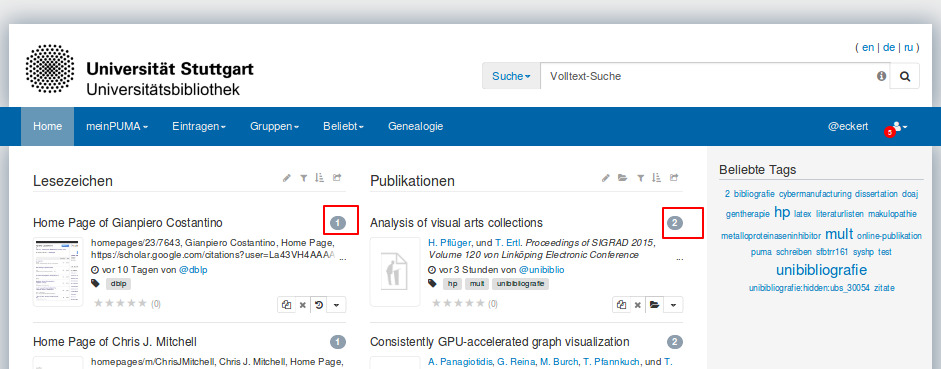
\includegraphics[width=10cm]{Bilder/Kapitel6/Duplikate}}
 \caption{Duplikate}
 \label{figure027}
\end{figure}
\subsection{Private Dateien anhängen}
Sie können an jede Ihrer Publikationen ein Dokument\index{Dokumente! anhängen} anhängen (max. 50 MB pro Datei - erlaubte Dateiendungen: pdf, ps, djv, djvu, txt, tex, doc, docx, ppt, pptx, xls, xlsx, ods, odt, odp, jpg, jpeg, svg, tif, tiff, png, htm, html, epub). Der Anhang ist aus urheberrechtlichen Gründen nur für Sie selbst sichtbar.

\begin{mdframed}[style=mdfexample1,frametitle={\texttt{BEDINGUNG}},backgroundcolor=gray!40]\texttt{Um an eine Publikation eine Datei anzuhängen, muss die Publikation in Ihrer Sammlung eingetragen sein.}\end{mdframed}
\begin{enumerate}
    \item Klicken Sie auf den Titel der Publikation. Es öffnet sich die Detailansicht der Publikation.
    \item Klicken Sie nun entweder auf den schwarzen Stift oben rechts auf der Seite. Es öffnet sich eine neue Seite, auf der Sie die Publikation bearbeiten können. Scrollen Sie runter bis zu \enquote{private Dokumente} und klicken auf \enquote{Durchsuchen}. \newline \textbf{ODER:} Sie klicken in der Detailansicht auf das Bild der Publikation. Unterhalb des Bildes erscheint der Durchsuchen-Button. 
    \item Es öffnet sich ein Pop-Up Fenster, indem Sie das Dokument auswählen können, welches Sie anhängen wollen. Klicken Sie anschließend auf \enquote{Öffnen}.
    \item Der Upload startet automatisch. Sobald er abgeschlossen ist, wird der Dateienname der hochgeladenen Datei und ein schwarzes \enquote{X} unter dem Abschnitt \enquote{private Dokumente} angezeigt. Über das schwarze \enquote{X} kann das Dokument wieder entfernt werden.
    \item Klicken Sie anschließend ganz unten auf der Seite auf \enquote{Speichern}, da ansonsten Ihre Änderung nicht gespeichert wird.
\end{enumerate}
\begin{figure}[h!]
 \centering
 \fbox{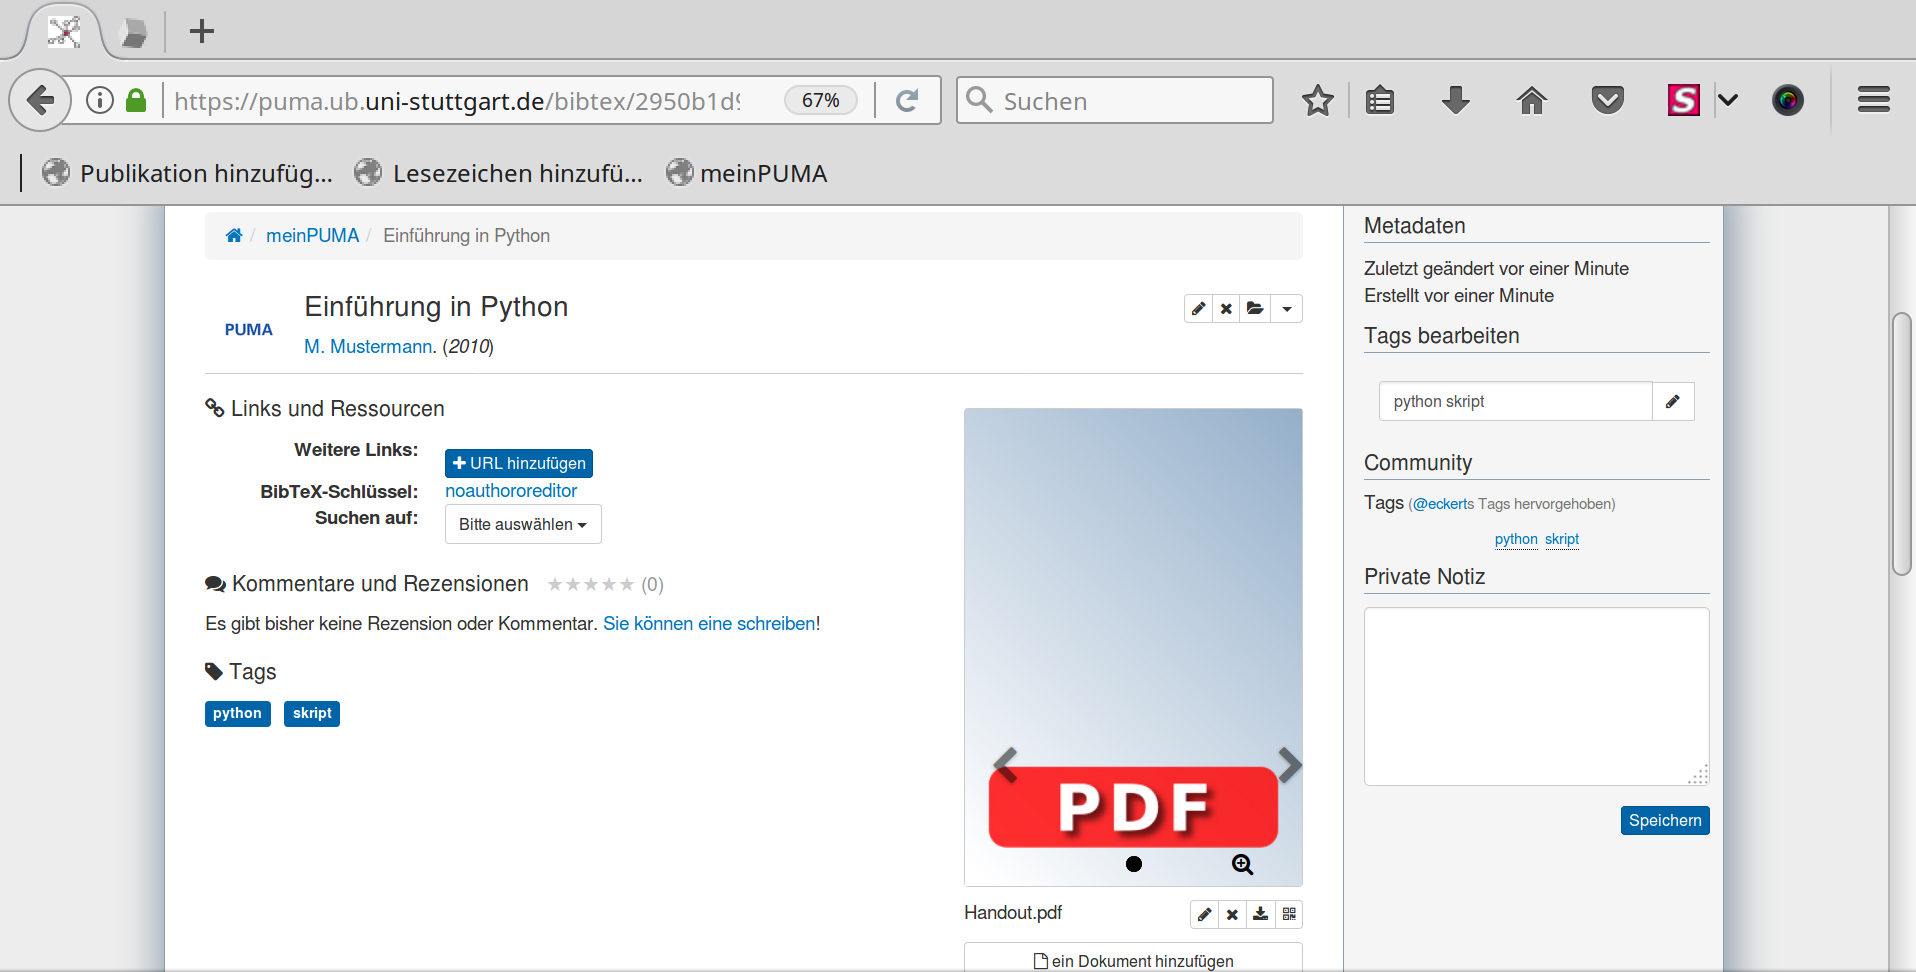
\includegraphics[width=10cm]{Bilder/Kapitel6/Private_Dokumente}}
 \caption{Private Dokumente anhängen}
 \label{figure028}
\end{figure}
Wenn die angehängte Datei auch für Gruppenmitglieder sichtbar seien soll, muss der  Gruppenadministrator das Teilen von Dokumenten erlauben
und die einzelnen Mitglieder dies ebenfalls in ihrer Gruppeneinstellung freischalten. In den Einstellungen kann der Nutzer unter dem Reiter \enquote{Gruppen} für jede einzelne Gruppe festlegen, ob Dateien geteilt werden oder nicht. Diese Funktion kann jederzeit wieder deaktiviert werden.
\subsection{Publikationen durchstöbern}
Oftmals verliert man schnell den Überblick über seine Einträge. Um sich schnell einen Überblick über seinen Literaturbestand machen zu können bietet PUMA die Funktion \enquote{Publikation\index{Publikationen!durchstöbern} durchstöbern} an. 
\begin{enumerate}
    \item Klicken Sie im Hauptmenü auf \enquote{meinPUMA}. Ein Dropdown-Menü öffnet sich.
    \item Klicken Sie auf \enquote{Publikationen durchstöbern}.
    \item Unter \enquote{Suchoptionen} können Sie verschiedene Tags und Autoren auswählen, zu denen Sie die Einträge sehen möchten. Um mehrere Begriffe aus der Liste auszuwählen, halten Sie die STRG- bzw. CTRL-Taste während des Mausklicks gedrückt.
\begin{figure}[h!]
 \centering
 \fbox{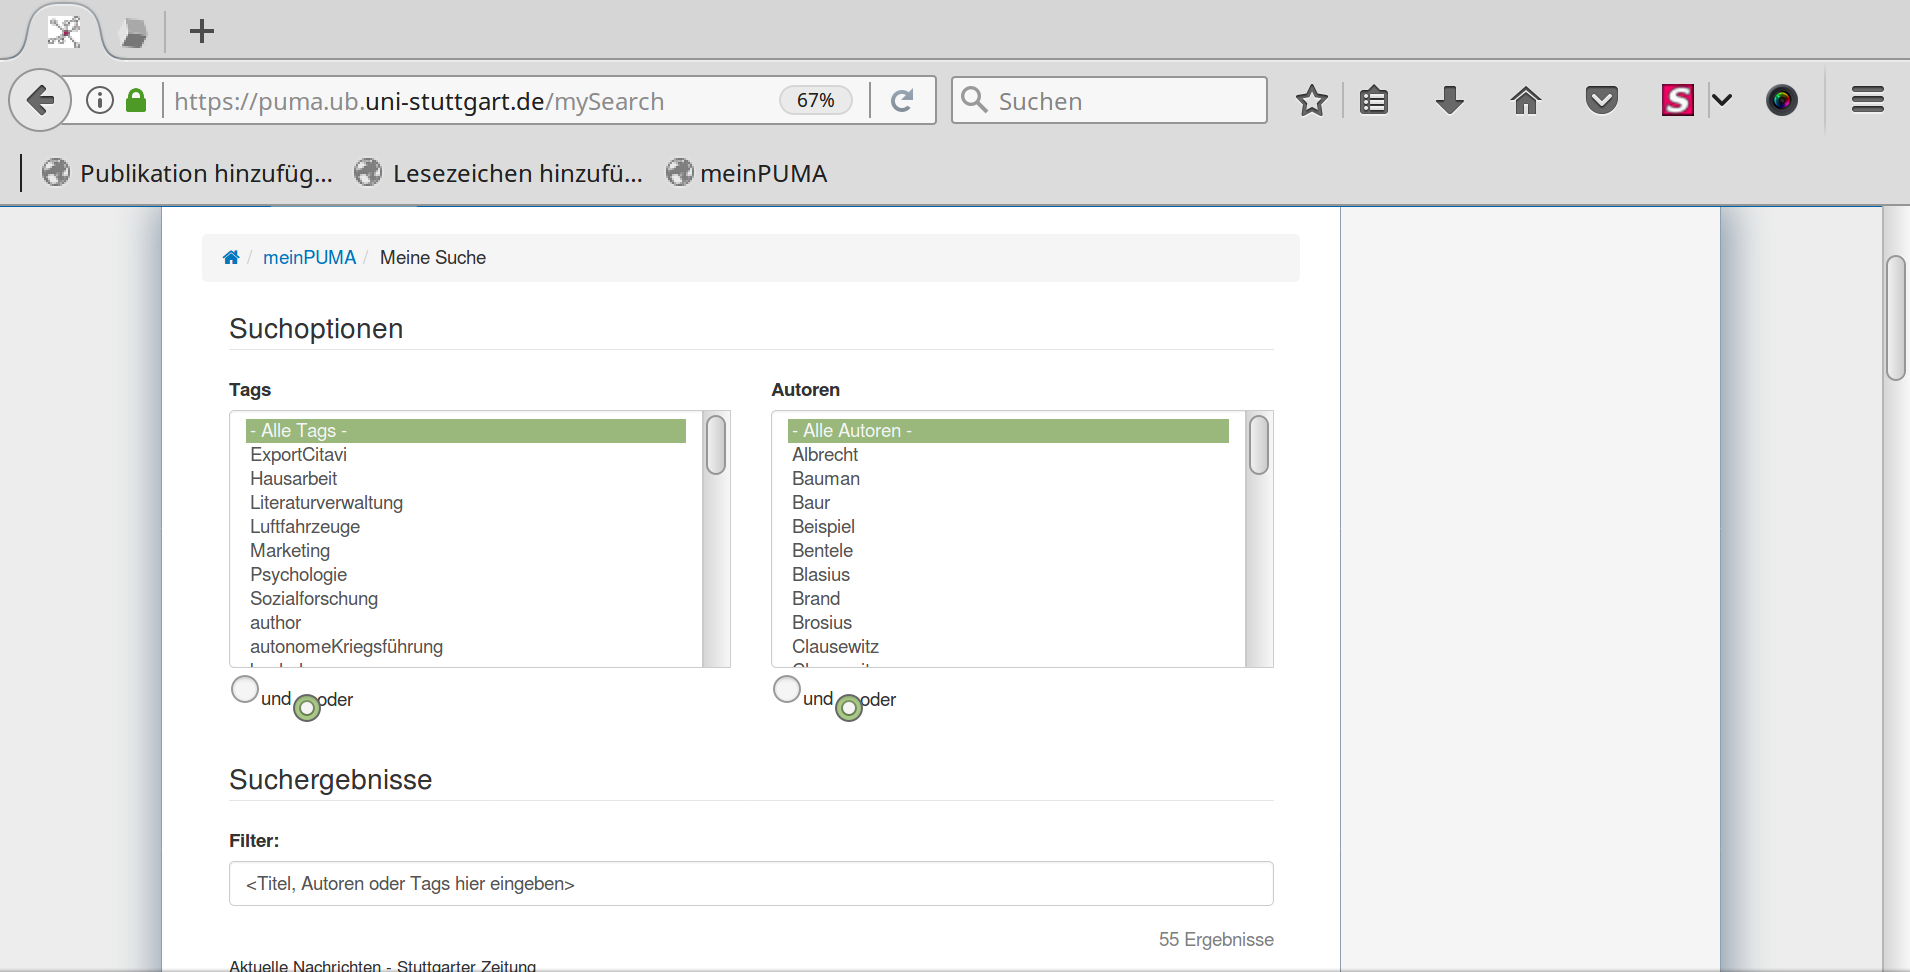
\includegraphics[width=10cm]{Bilder/Kapitel6/Publikationen_durchstoebern}}
 \caption{Publikationen durchstöbern}
 \label{figure029}
\end{figure}
    \item Die Buttons \enquote{und/~oder} können Sie dazu nutzen, um die Listenauswahl unterschiedlich zu verknüpfen. 
    \item Unter \enquote{Suchergebnisse} sehen Sie alle Ergebnisse, die zu ihren Vorgaben aus 3. und 4. passen.
    \item Das Textfeld \enquote{Filter} ermöglicht es die Ergebnisse aus Schritt 5 noch weiter zu filtern.
\end{enumerate}
\subsection{Eigene Einträge bearbeiten}
Ist ein Eintrag einmal hinzugefügt, heißt dies nicht, dass man ihn nie mehr bearbeiten kann. Die erste Möglichkeit wäre, dass der Nutzer jeden Eintrag selber von Hand nachträglich bearbeitet. Die zweite Lösung ist zeitsparender und schneller.\newline
In der Sammlung befindet sich oben rechts oberhalb der Publikations- und Lesezeichenspalte ein Stift, mit dem Sie Ihre eigenen Eintrage bearbeiten können. Durch das Klicken auf den Stift gelangen Sie auf die Seite \enquote{Eigene Einträge bearbeiten}. Hier können Sie auswählen, was Sie an der/~den Publikation/~en ändern möchten:
\begin{itemize}
\item Tags zu allen ausgewählten Posts hinzufügen
\item Die Tags aller ausgewählten Einträge separat bearbeiten
\item BibTex-Schlüssel normalisieren
\item Einträge löschen
\item Sichtbarkeit einstellen
\end{itemize}
Die Änderungen können für eine Publikation/Lesezeichen oder mehrere sein. Dies können Sie unten auf der Seite festlegen. Durch klicken auf die entsprechenden Einträge wählen Sie diese aus.
\begin{figure}[h!]
 \centering
 \fbox{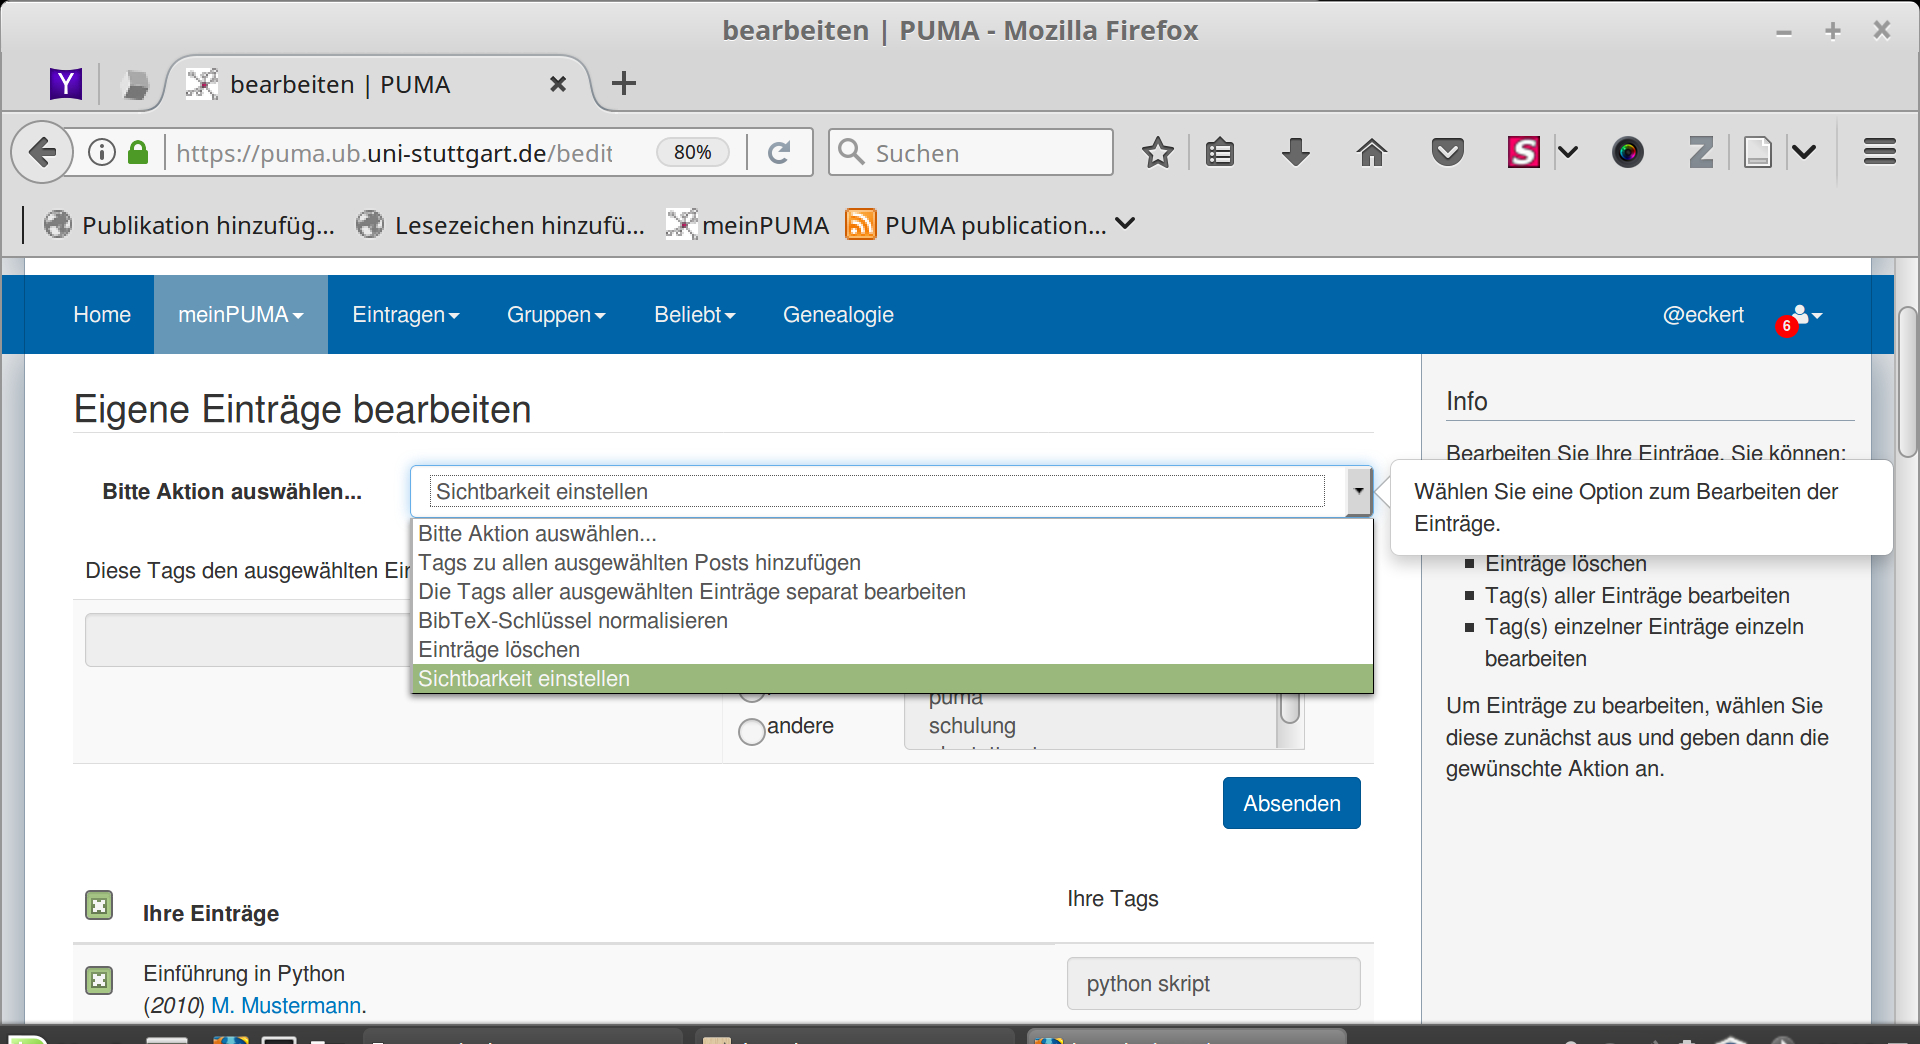
\includegraphics[width=10cm]{Bilder/Kapitel6/Eigene_Eintraege_bearbeiten}}
 \caption{Eigene Einträge bearbeiten}
 \label{figure030}
\end{figure}
\subsection{OpenURL-Resolver/Bestandsanfrage}
\label{subsec:OpenURL}
Mit Hilfe von OpenURL\index{OpenURL} kann man bei Publikationen aus seiner eigenen Sammlung überprüfen, ob sich diese im Katalog der jeweiligen Büchereien befindet. Dafür müssen Sie  die folgende URL:  
\url{http://www.redi-bw.de/links/unist} in Ihre Einstellungen kopieren, dabei gehen Sie wie folgt vor:
\begin{enumerate}
    \item Klicken Sie auf das Personensymbol, ein Untermenü öffnet sich.
    \item Klicken Sie auf \enquote{Einstellungen}.
    \item Geben Sie in der Rubrik \enquote{Kontakt} in das Feld \enquote{OpenURL} die URL \url{http://www.redi-bw.de/links/unist} ein. 
\begin{figure}[h!]
 \centering
 \fbox{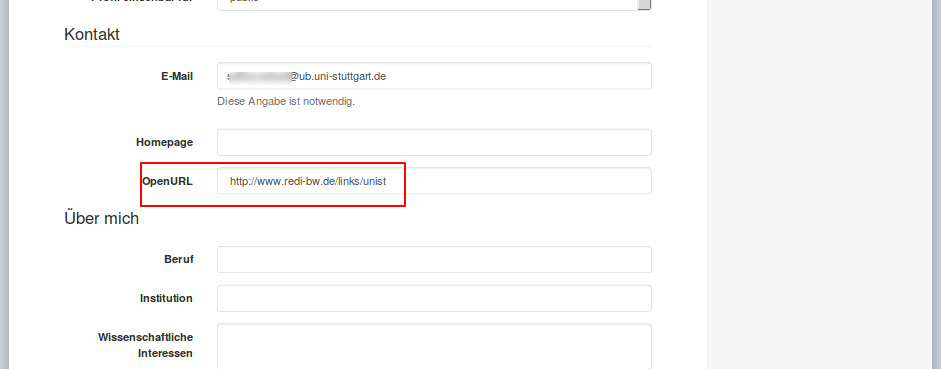
\includegraphics[width=10cm]{Bilder/Kapitel6/Open_URL}}
 \caption{Open-URL der Universität Stuttgart}
 \label{figure031}
\end{figure}
    \item Speichern Sie die Änderung auf dem Ende der Seite.
\end{enumerate}
Ab sofort befindet sich bei jeder Ihrer Publikationen unter dem Bereich \enquote{Links und Ressourcen} die entsprechende Open-URL, über die Sie nun eine Bestandsabfrage durchführen können.
\begin{figure}[h!]
 \centering
 \fbox{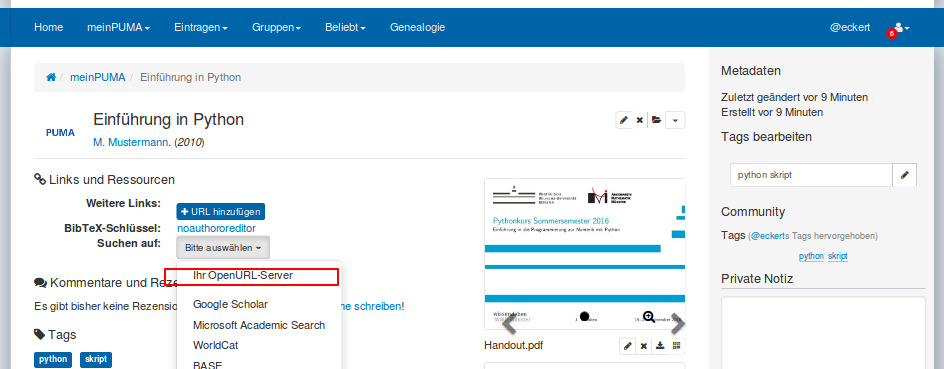
\includegraphics[width=10cm]{Bilder/Kapitel6/OpenURL-Resolver}}
 \caption{OpenURL-Resolver}
 \label{figure032}
\end{figure}
\subsection{Open Access-Zugriff auf Publikationsdienste}%Screenshot
Der Zugriff auf Open Access\index{Open Access} Publikationsdienste ermöglicht Ihnen über die Detailansicht einer Publikation nach der digitalen Ausgabe in einer Open Access-Datenbank zu suchen. Voraussetzung hierfür ist, dass die Detailansicht der Publikation aufgerufen ist. Zur Detailansicht gelangen Sie, indem Sie im Inhaltsbereich oder Ihrer persönlichen Sammlung (unter \enquote{Mein PUMA}) auf den Titel einer Publikation klicken. 
\begin{enumerate}
    \item Klicken Sie auf das Auswahlmenü \enquote{Suchen auf}. Ein Untermenü erscheint.
\begin{figure}[h!]
 \centering
 \fbox{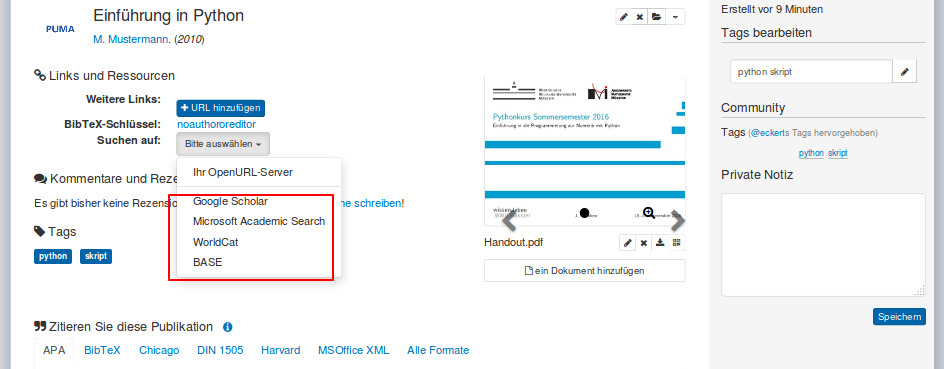
\includegraphics[width=10cm]{Bilder/Kapitel6/Open-Access}}
 \caption{Open Access}
 \label{figure033}
\end{figure}
    \item Wählen Sie aus der angezeigten Liste die Open Access-Datenbank, die Sie nach diesem Artikel durchsuchen möchten. 
\end{enumerate}
 So gelangen Sie schnell und einfach zu der digitalen Ausgabe einer Publikation. 
\subsection{Eingang}
In Ihrem Eingang\index{Eingang} finden Sie alle Beträge, die Ihnen von Freunden geschickt wurden.
\begin{figure}[h!]
 \centering
 \fbox{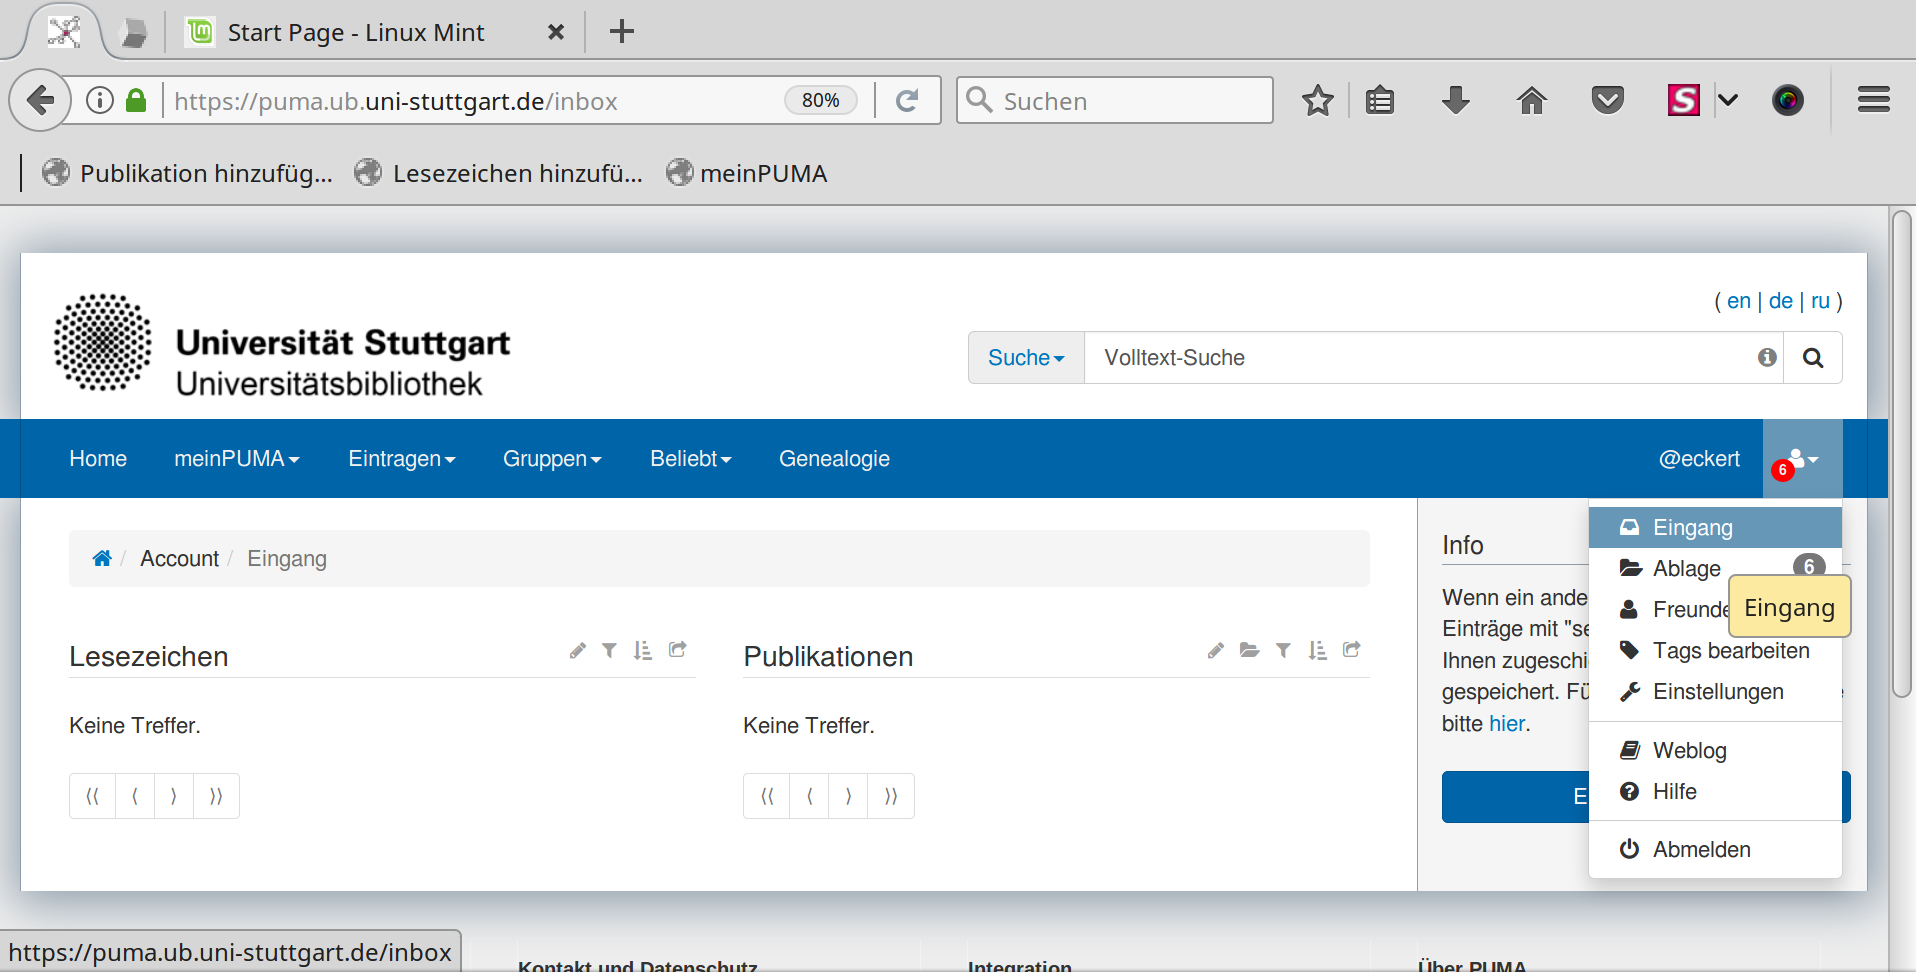
\includegraphics[width=10cm]{Bilder/Kapitel6/Eingang}}
 \caption{Der Eingang}
 \label{figure034}
\end{figure}
\underline{Einträge verschicken\index{Einträge!verschicken}}
\newline
Um einem anderen Nutzer ein Lesezeichen oder eine Publikation zu schicken, verwenden Sie das Systemtag \textit{send:xyz}. Dieses Tag geben Sie mit weiteren Tags beim Eintragen einer Publikation/Lesezeichen mit ein. Der Eintrag wird dann getaggt mit from:<YourUserName> und in den Eingang von dem Nutzer xyz kopiert. Um den Missbrauch des Eingangs zu verhindern, muss der Empfänger des Eintrags
\begin{enumerate}
    \item entweder mit Ihnen befreundet sein
    \item oder Mitglied einer gemeinsamen Gruppe sein.
\end{enumerate}
Nachdem der Eintrag gesendet wurde wird der Tag von \textit{send:xyz} in \textit{sent:xyz} automatisch umgewandelt.
\newline
\newline
\underline{Einträge erhalten\index{Einträge!erhalten}}
\newline
In Ihrem Eingang liegen alle Einträge, die Ihnen geschickt wurden. Sie können diese Einträge über den Button \enquote{Diese Publikation in die eigene Sammlung einfügen}, rechts neben dem Eintrag (zwei Blätter) übernehmen. Mit \enquote{Diese Publikation aus Ihrem Eingang entfernen} können Sie den Eintrag aus dem Eingang löschen und über das schwarze Zahnrad den ganzen Eingang leeren.
\section{Literaturlisten erstellen}
PUMA bietet Ihnen die Möglichkeit, aus Ihren gesammelten Publikationen Literaturlisten\index{Literaturlisten} zu erstellen, die Sie später beispielsweise auf externen Webseiten verwenden können. \newline
Hierfür fügen Sie die Publikationen, die in das Literaturverzeichnis sollen, zu Ihrer Ablage\index{Ablage} hinzu. Wenn Sie alle Publikationen hinzugefügt haben, klicken Sie in der Ablage, oberhalb von den Publikationen, auf Exportzeichen und wählen Sie \enquote{mehr...} aus. Sie gelangen nun zu einer Übersichtsseite, auf der Ihnen alle verfügbaren Zitationsstile angezeigt werden, und Sie nur noch den passenden aussuchen müssen. 
\subsection{Eigene Literaturlisten erstellen} 
Neben den Layouts für das Erstellen einer Literaturliste können Sie auch folgenden URLs verwenden, die Sie in Ihren Browser eingeben:
\begin{enumerate}%Beispielscreenshots ?
    \item \textbf{Allgemeine Liste:}\newline
    \textit{https://puma.ub.uni-stuttgart.de/publ/user/<username>} \newline
    Ersetzen Sie \textit{<username>} durch Ihren Benutzernamen und Ihnen werden alle Publikationen aus Ihrer Sammlung in einer Literaturliste angezeigt.\newline
    \textbf{Beispiel:} https://puma.ub.uni-stuttgart.de/publ/user/eckert 
\begin{figure}[h!]
 \centering
 \fbox{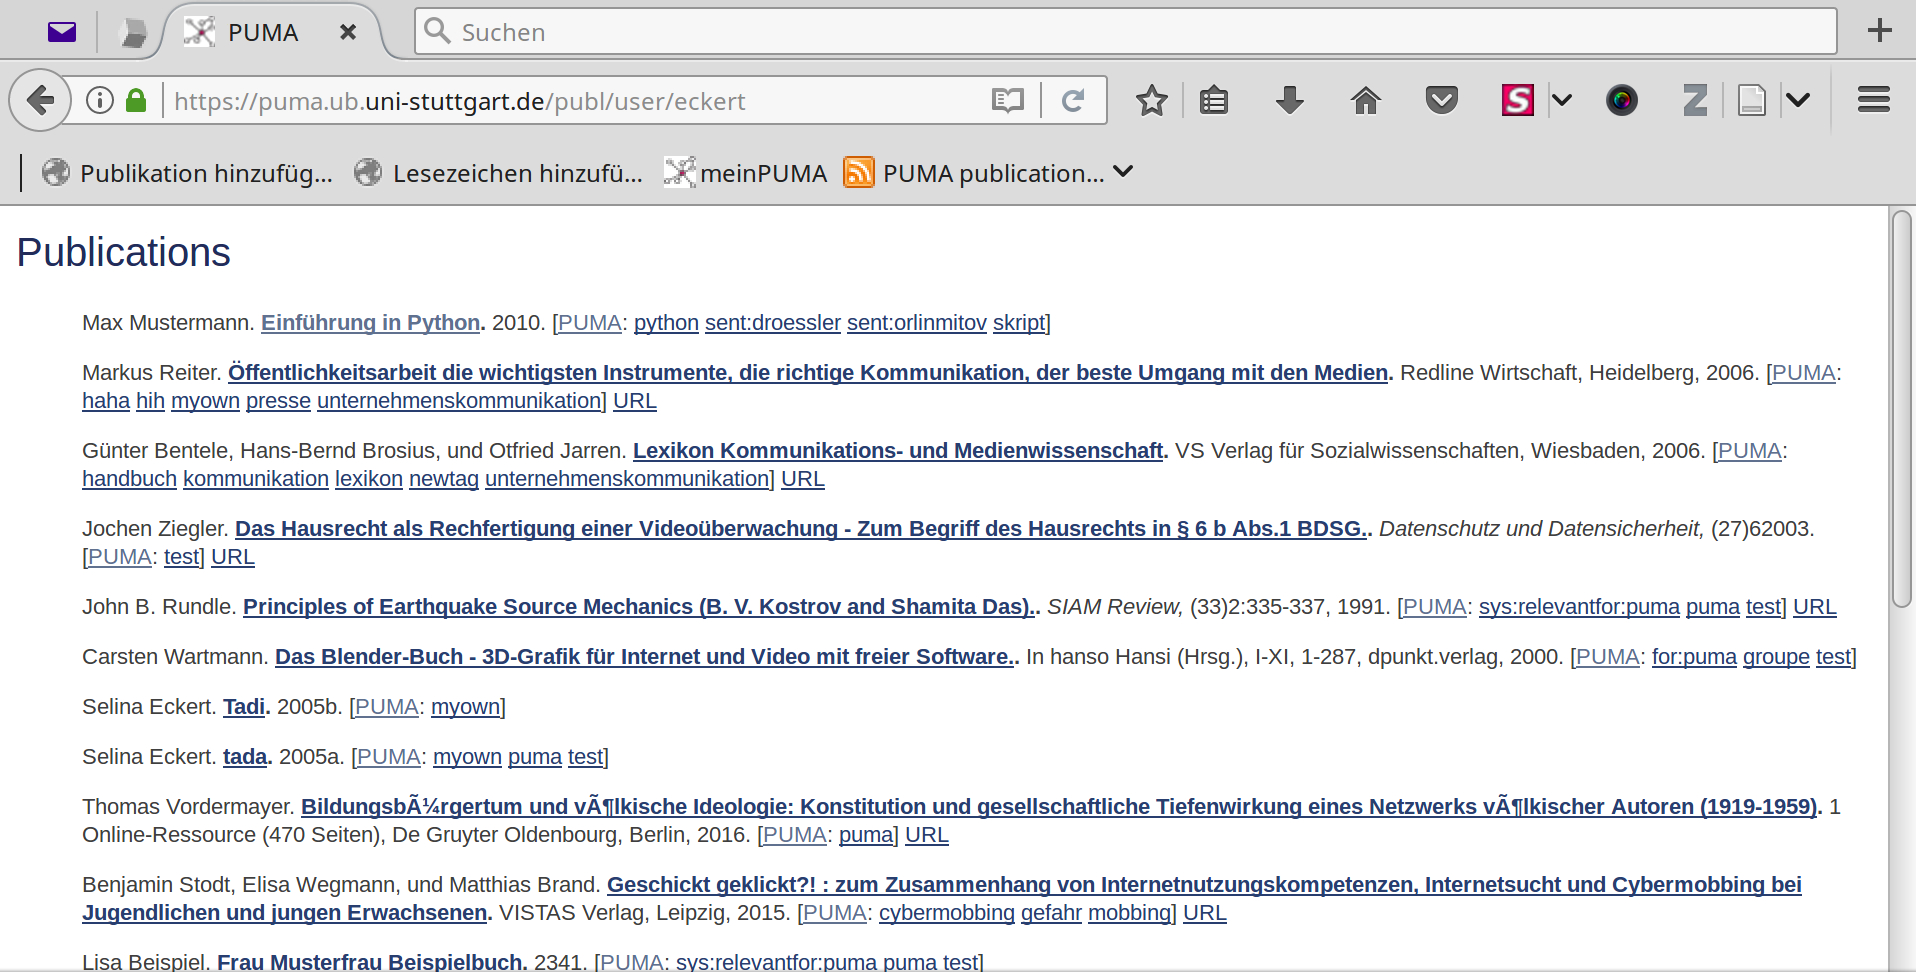
\includegraphics[width=11cm]{Bilder/Kapitel6/Allgemeine_Liste}}
 \caption{Allgemeine Liste}
 \label{figure035}
\end{figure}

    \item \textbf{Allgemeine Liste ohne Tags:}\newline
    \textit{https://puma.ub.uni-stuttgart.de/publ/user/<username>?notags=1}\newline
    Ersetzen Sie \textit{<username>} durch Ihren Benutzernamen und Ihnen werden alle Publikationen aus Ihrer Sammlung, ohne Tags, in einer Literaturliste angezeigt.\newline
    \textbf{Beispiel:} https://puma.ub.uni-stuttgart.de/publ/user/eckert?notags=1 
    
\begin{figure}[h!]
 \centering
 \fbox{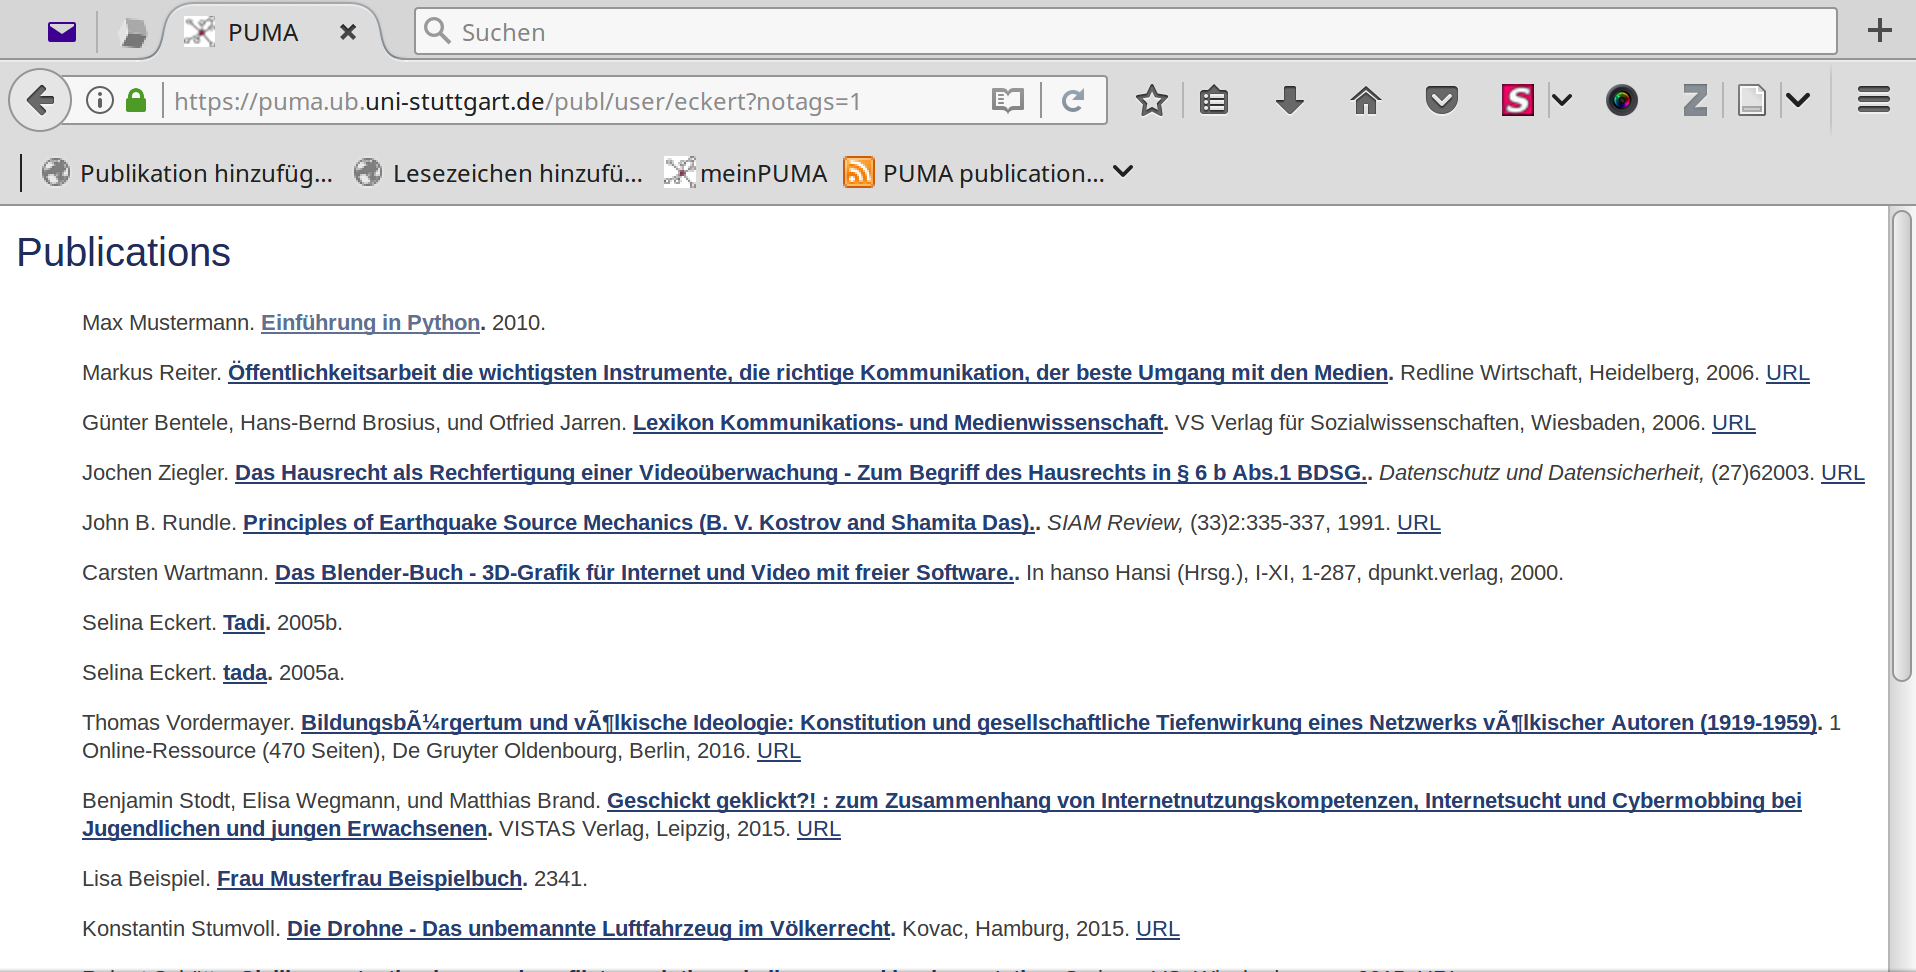
\includegraphics[width=11cm]{Bilder/Kapitel6/Allgemeine_Liste_ohne_Tags}}
 \caption{Allgemeine Liste ohne Tags}
 \label{figure036}
\end{figure}

    \item \textbf{Allgemeine Liste mit Tag-Einschränkung:}\newline
    \textit{https://puma.ub.uni-stuttgart.de/publ/user/<username>/<tagname>}\newline
    Ersetzen Sie \textit{<username>} durch Ihren Benutzernamen und \textit{<tagname>} durch den Tag, der in den Publikationen enthalten sein soll. Ihnen wird eine Literaturliste angezeigt, die jene Publikationen aus Ihrer Sammlung enthält, die den speziellen Tag enthalten. Ein besonderes Beispiel hierfür ist der Tag \textit{myown\index{myown}}. Durch diesen Tag geben Sie an, dass Sie der/~die Verfasser/~in der Publikation sind. \newline
    \textbf{Beispiel:} https://puma.ub.uni-stuttgart.de/publ/user/eckert/puma
   
\begin{figure}[h!]
 \centering
 \fbox{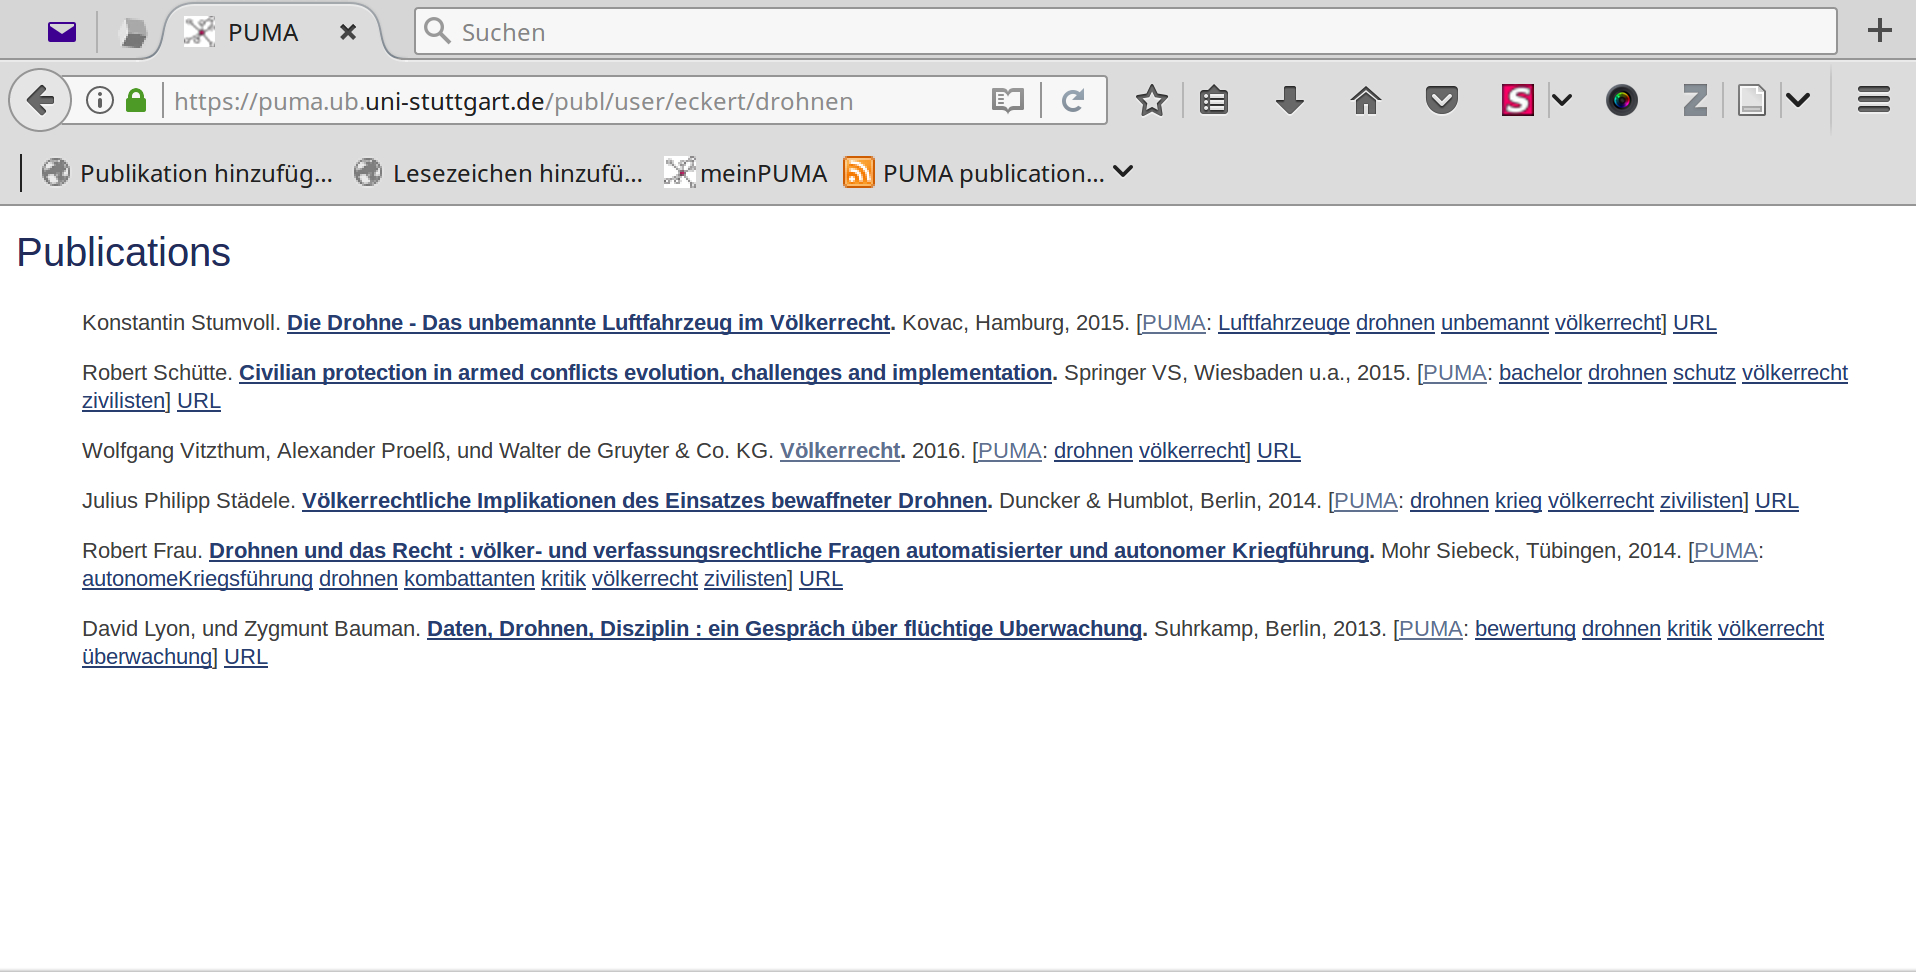
\includegraphics[width=11cm]{Bilder/Kapitel6/Allgemeine_Liste_Tag_Einschraenkung}}
 \caption{Liste mit Tagauswahl}
 \label{figure037}
\end{figure}

    \item \textbf{BibTeX-Liste:}\newline
    \textit{https://puma.ub.uni-stuttgart.de/bib/user/<username>} \newline
    Ersetzen Sie \textit{<username>} durch Ihren Benutzernamen. Ihnen wird eine Literaturliste mit all Ihren Publikationen im BibTex-Format\index{BibTex} angezeigt.\newline
    \textbf{Beispiel:} https://puma.ub.uni-stuttgart.de/bib/user/eckert 

\begin{figure}[h!]
 \centering
 \fbox{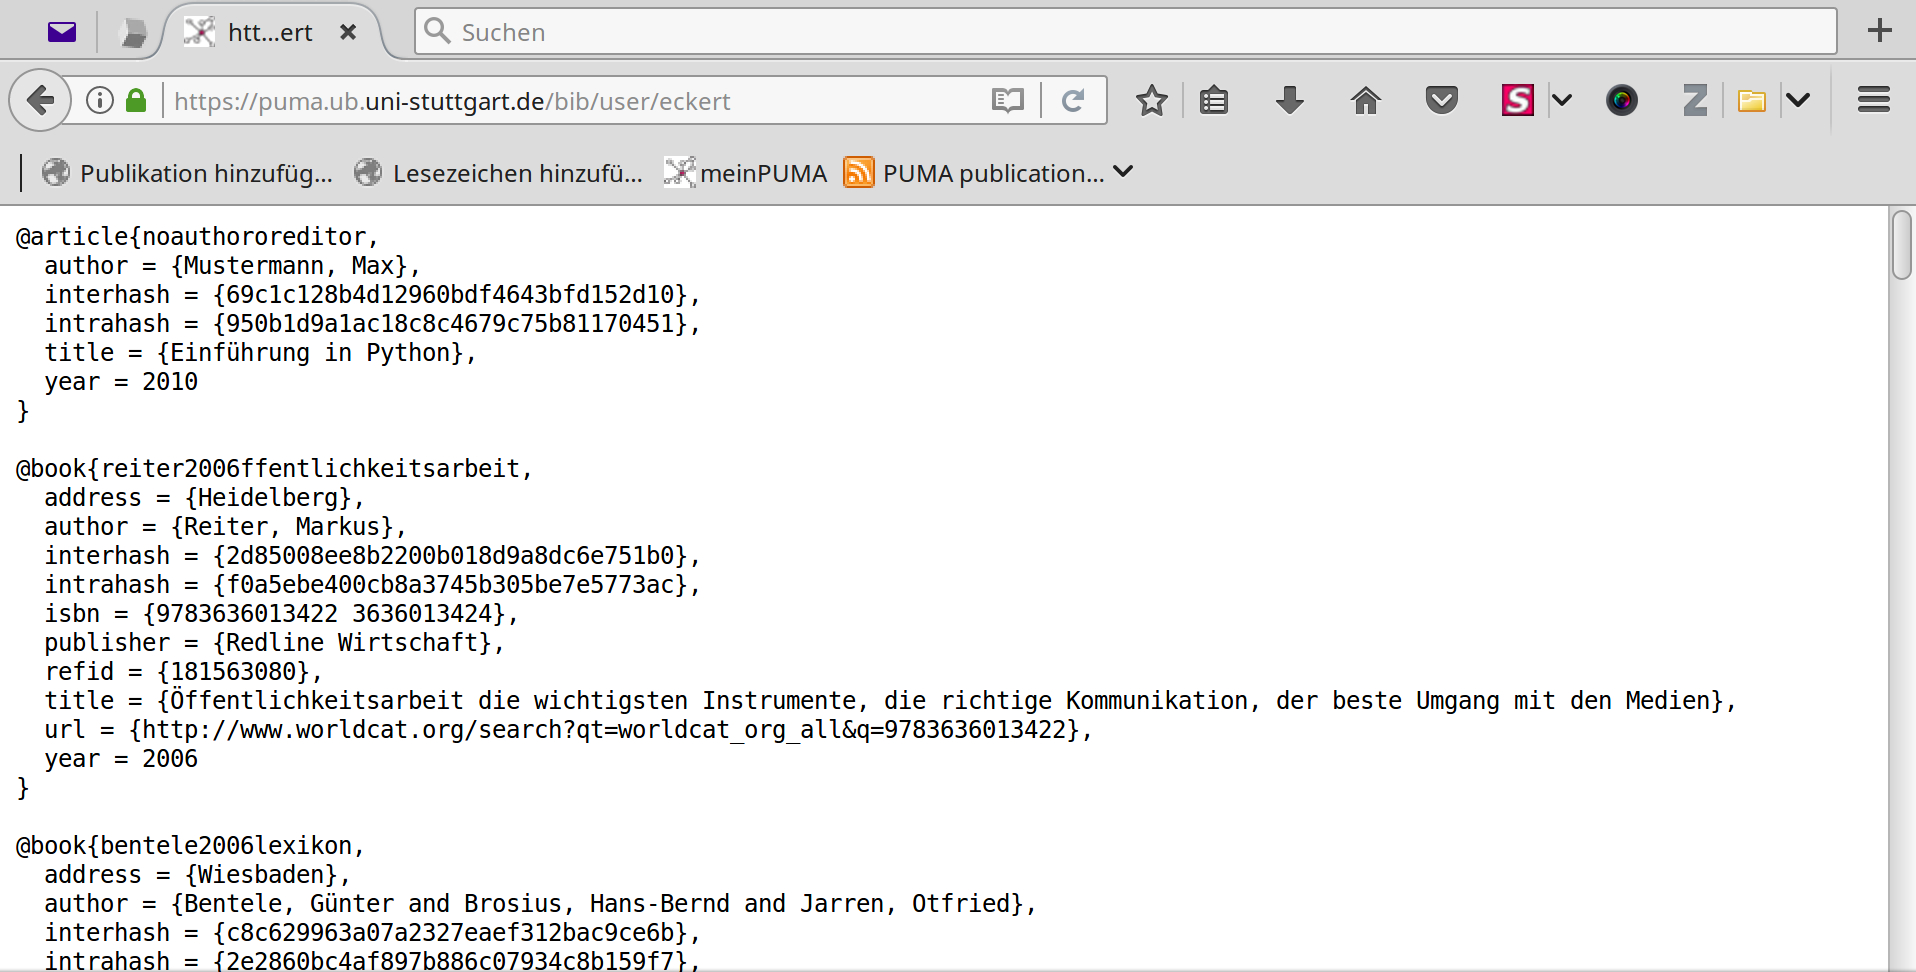
\includegraphics[width=11cm]{Bilder/Kapitel6/Bibtex_Liste}}
 \caption{BibTex-Liste}
 \label{figure038}
\end{figure}

\end{enumerate}
\subsection{JabRef-Layouts}
Einen kompletten Überblick zu allen verfügbaren Jabref-Layouts\index{JabRef!Layouts} erhalten Sie auf der Export-Seite von PUMA.
\begin{enumerate}
	\item  \textbf{/layout/simplehtml/}\newline
	Sie erhalten eine HTML-Übersicht - über alle Publikationen im 		Inhaltsbereich - ohne Kopf- oder Fußzeile nützlich für die 			Einbindung von Publikationslisten in andere HTML-Seiten.
	\item \textbf{/layout/html/}\newline
    Eine einfache Übersicht aller Publikationen aus dem Inhaltsbereich, in der jeder Eintrag als Zeile in einer Tabelle dargestellt ist.
	\item \textbf{/layout/tablerefs/} \newline
    HTML-Ausgabe mit jedem Eintrag als Zeile in einer Tabelle und einer zusätzlichen JavaScript-Suchfunktion.
\item \textbf{/layout/tablerefsabsbib/} \newline
    Ähnelt \textit{/layout/tablerefs/}. Enthält auch die BibTeX-Quelle und die Kurzbeschreibung der Publikation.
\item \textbf{/layout/docbook/} \newline
    Dies ist eine XML-Ausgabe gemäß dem DocBook-Schema.
\item \textbf{/layout/endnote/} \newline
    Sie erhalten eine Ausgabe in RIS, welche von dem Literaturverwaltungsprogramm EndNote verwendet wird.
\item \textbf{/layout/dblp/} \newline
    DBLP exportiert alle Publikationen aus dem Inhaltsbereich in eine DBLP-konforme XML-Struktur. 
\item \textbf{/layout/text/}\newline
    Alle Publikationen aus dem Inhaltsbereich werden in einer BibTeX-Ausgabe dargestellt.
\end{enumerate}

\todo[inline]{Sortieren: Datum! Bibtexfelder auswählen Persönlicher Bereich vs. Lucine Index}
\todo[inline]{Dubletten erklären}
